\documentclass[fleqn]{article}

\usepackage[utf8]{inputenc}
\usepackage{fullpage}
\usepackage{graphicx}
\usepackage{amsmath}
\usepackage{amssymb}
\usepackage{mathbbol}
\usepackage{chngcntr}
\usepackage{hyperref}
\usepackage{tcolorbox}
\usepackage{subcaption}

\DeclareMathOperator{\E}{\mathop\mathbb{E}}
\DeclareMathOperator{\V}{\mathbb{Var}}
\DeclareMathOperator{\B}{\mathbb{Bias}}
\counterwithin*{equation}{subsection}
\counterwithin*{equation}{section}

\newcommand{\independent}{\perp \!\!\! \perp}
\newcommand{\indepg}{\perp \!\!\! \perp_G}
\def\define#1{\textbf{def} \textbf{#1}}
\newtheorem{theorem}{Theorem}
\newtheorem{lemma}{Lemma}
\newtheorem{corollary}{Corollary}

\DeclareMathOperator*{\argmin}{argmin}
\DeclareMathOperator*{\argmax}{argmax}

\numberwithin{equation}{section}
\numberwithin{theorem}{section}
\numberwithin{figure}{section}
\numberwithin{lemma}{section}
\numberwithin{corollary}{section}

\title{Causal Inference Notes}
\author{Andrei Serebro}

\begin{document}
	
	
	\section{Introduction}
	Notes from reading Judea Pearl's book "Causality: Models, Reasoning and Inference".
	
	\section*{Introduction to Probabilities, Graphs, and Causal Models}
	
	What is the connection between causality and probability theory? There are two main reasons.
	
	First, statements about causes and effects typically come with some degree of uncertainty. Often, causes don't make their effects absolutely certain, but only increase their probability.
	
	Second (which is closely related to the first), even seemingly obvious cause-effect relationships hold only \textit{almost always}: there are many small details that are difficult to account for.
	
	Consider the factorization of a distribution $P(x_1,...x_N) = \prod\limits_{n}P(x_n|x_1...x_{n-1})$.
	
	\define{Markovian parents} of a random variable $X_n$ are the minimal subset of variables $PA_n \subset \{X_1...X_{n-1}\}$ such that $P(x_n|pa_n) = P(x_n|x_1..x_{n-1})$.
	
	\define{Bayesian network} is a DAG constructed with variable vertices and edges connecting each vertex to its Markovian parents (edges are directed from parents to children).
	
	It can be shown that given an ordering of variables, the Markovian parents for each variable are uniquely determined if the distribution $P(X_1,...X_N)$ is strictly positive, meaning any variable combination has probability $>0$ (unless it contains values whose marginal probability equals 0). This is a sufficient condition for the conditional probabilities $P(x_n|x_1..x_{n-1}) = \frac{P(x_1, ..., x_n)}{P(x_1,..,x_{n-1})}$ to be well-defined, since the denominator never becomes zero within the domain of $P(x_1,...,x_N)$.
	
	\define{Markov Compatibility} A distribution $P$ is said to be Markov compatible with DAG $G$ if it factorizes according to the graph, i.e., $P(x) = \prod\limits_n P(x_n|pa_n)$.
	
	A convenient way to characterize distributions $P$ compatible with $G$ is through the list of independencies that must hold in these distributions. These independencies can be determined graphically using the $d$-separation criterion (which can be found in Bishop), but for completeness:
	
	\define{$d$-separation} A path $p$ in DAG $G$ is said to be $d$-separated/blocked by a set of vertices $Z$ if at least one of three conditions holds:\\
	1. The path contains a chain $a\to b\to c$ where $b\in Z$\\
	2. The path contains a fork $b\to a, b\to c$ where $b\in Z$\\
	3. The path contains a $v$-structure where the collider is not in $Z$ and none of its descendants are in $Z$: $a\to b, c\to b, b \notin Z, de(b) \cap Z = \emptyset$
	
	\begin{figure}[h]
		\begin{center}
			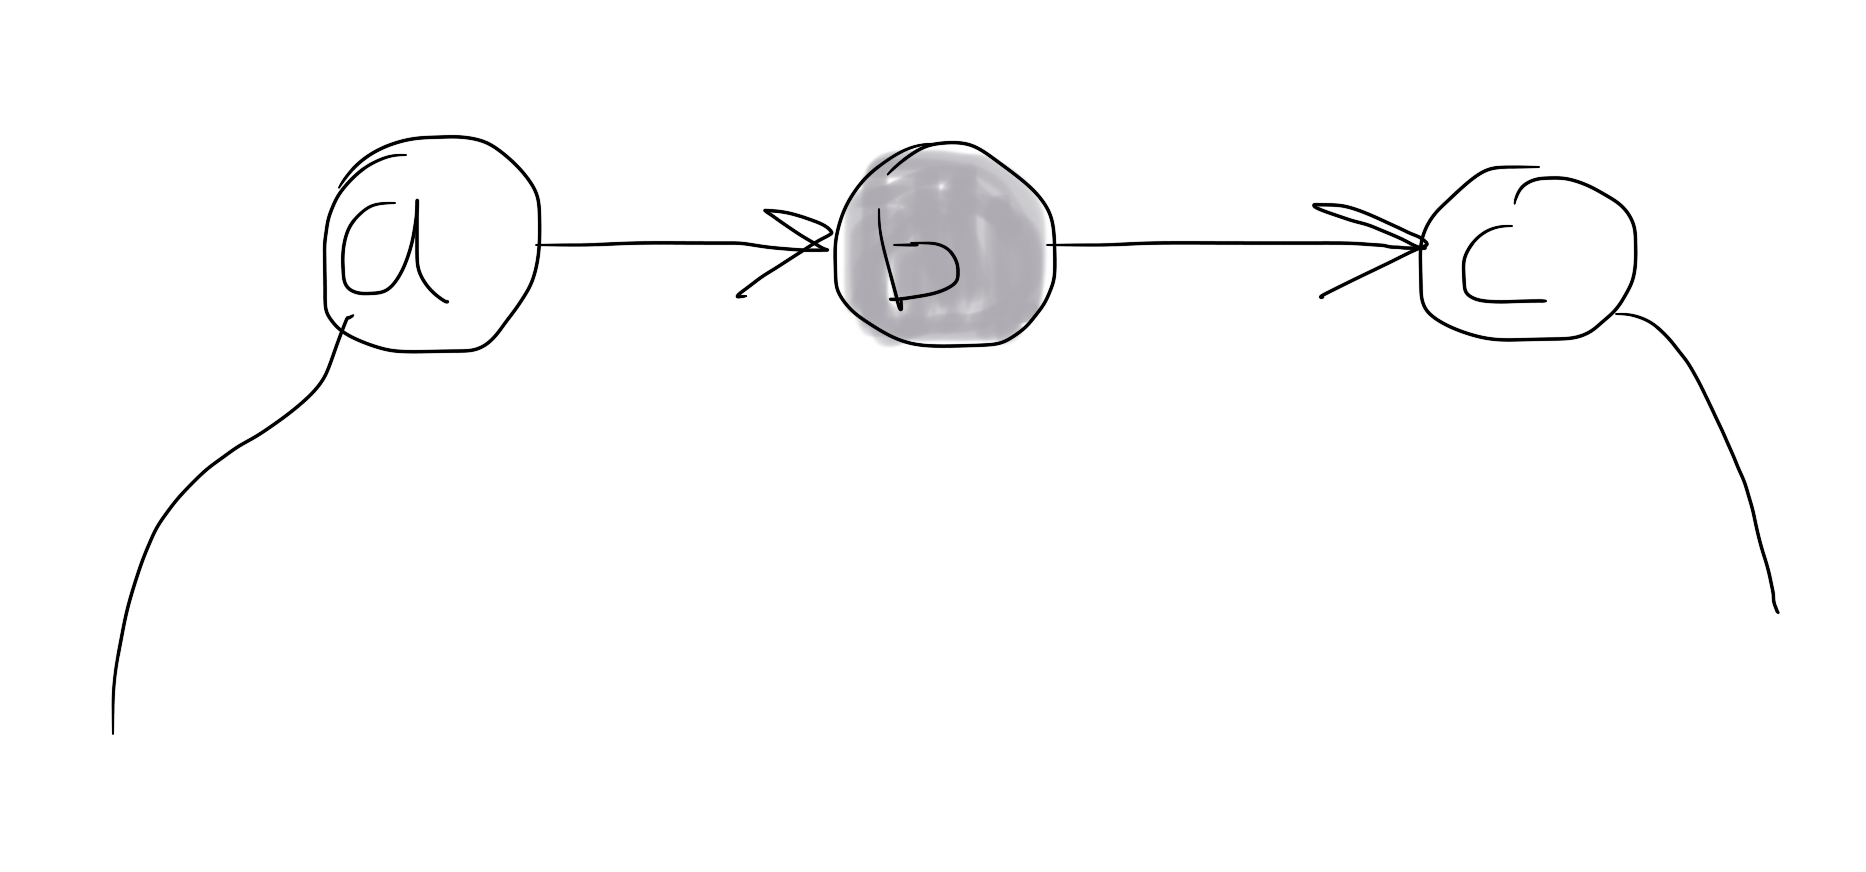
\includegraphics[scale=0.07]{imgs/img4.png}
			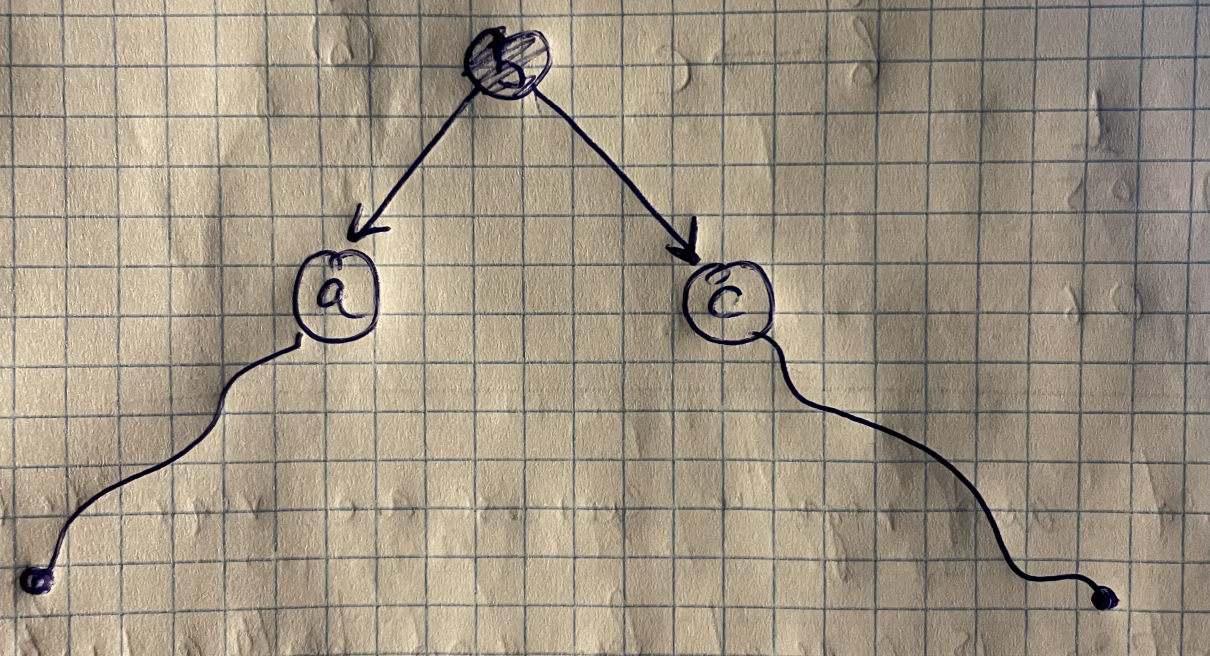
\includegraphics[scale=0.07]{imgs/img5.png}
			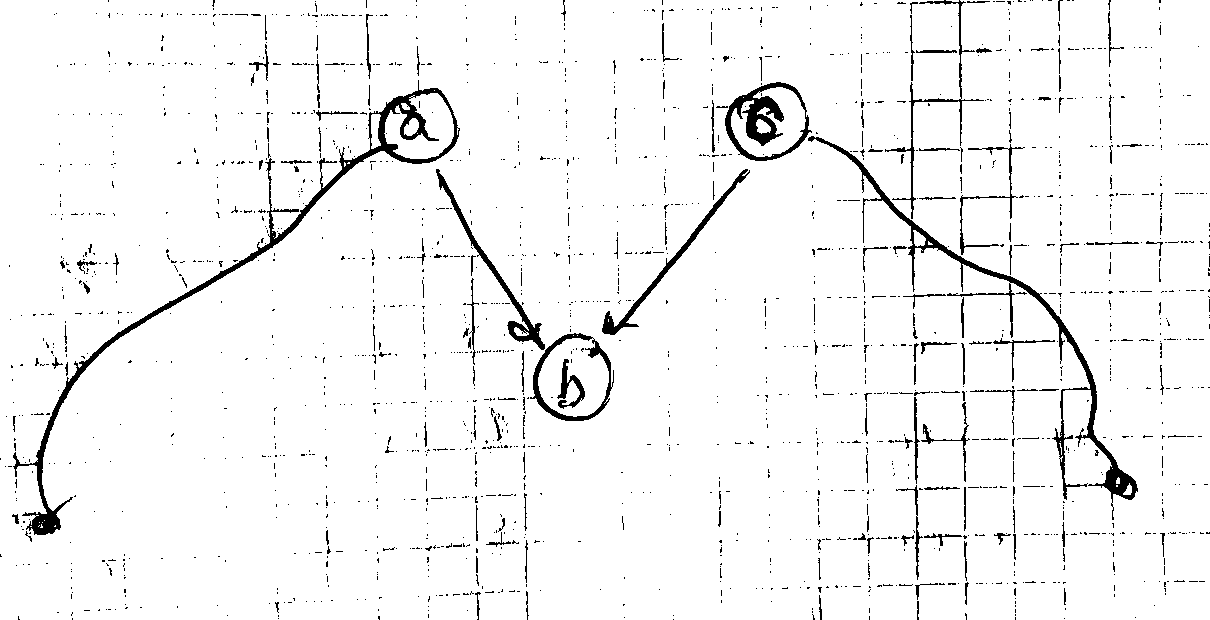
\includegraphics[scale=0.08]{imgs/img6.png}
		\end{center}
		\caption{Various cases of $d$-separation, shaded vertices $\in Z$}
		\label{fig:dsep1}
	\end{figure}
	
	A set $Z$ $d$-separates sets $X$ and $Y$ if it blocks all paths between $X$ and $Y$.
	
	\subsection*{Applications of $d$-separation}
	
	Why did we introduce $d$-separation? Here's why:
	
	\begin{theorem} Probabilistic consequences of $d$-separation\\
		If sets $X$ and $Y$ are $d$-separated by set $Z$, then $X \independent Y\ |\ Z$ in any distribution compatible with $G$. Conversely, if $X$ and $Y$ are not $d$-separated by $Z$ in $G$, then there exists at least one compatible distribution where $X \not \independent Y \ | \ Z$.
		\label{th:th1}
	\end{theorem}
	
	Proof: We begin by introducing the concept of a semi-graphoid relation.
	
	\vspace{0.2cm}
	
	\define{Dependency model} is a ternary relation over subsets of $2^V$ of some set $V$, where triples are interpreted as independence statements between the first and third elements given the second.
	
	\define{Semi-graphoid} is the closure of a dependency model under the first four properties ($X, Y, Z, W$ are disjoint subsets of the carrier set $V$):
	\begin{tcolorbox}
		1. Symmetry: $I(X, Z, Y) \iff I(Y, Z, X)$ \\
		2. Decomposition: $I(X, Z, Y\cup W) \implies I(X, Z, Y)\ \&\ I(X, Z, W)$\\
		3. Weak union: $I(X, Z, Y\cup W) \implies I(X, Z \cup W, Y)$\\
		4. Contraction: $I(X, Z\cup Y, W)\ \&\ I(X, Z, Y) \implies I(X, Z, Y\cup W)$\\
		5. Intersection: $I(X, Z\cup Y, W)\ \&\ I(X, Z\cup W, Y) \implies I(X, Z, Y\cup W)$
	\end{tcolorbox}
	
If, in addition, the semi-graphoid is closed under the fifth property, it is called a \textbf{graphoid}.

An example of a semi-graphoid (and indeed, why they are interesting in this context), defined on the set of subsets of random variables \( V \), is the relation of conditional independence: \( I(X,Y,Z) \iff X \independent Y\ |\ Z \). If the distribution is also strictly positive, meaning that for any set of variable values \((x_1, \ldots, x_N)\): \(\forall i \in [1..N]\ \sum_{X_j, j \neq i} P(x_1, \ldots, x_N) > 0 \implies P(x_1, \ldots, x_N) > 0\), then the conditional independence relation will be a graphoid. Why is this condition important? Let's consider this when we prove property 5.

\vspace{0.2cm}

Let's prove this to warm up.

1. Symmetry is quite obvious: indeed, if \( P(X, Y | Z) = P(X | Z)P(Y|Z) \), then the symmetric statement is also true, since \( P(Y, X|Z) = P(X, Y|Z) = P(X|Z)P(Y|Z) = P(Y|Z)P(X|Z) \).

2. Decomposition: Let \( P(X, YW | Z) = P(X|Z)P(YW|Z) \). Then, simply sum the left and right sides over the set of values \( W \):

For the left side, we have \(\sum_{w} P(X, YW|Z) = P(X, Y|Z)\).

For the right side, similarly:

\begin{align}
	\sum_{w} P(X|Z)P(YW|Z) = P(X|Z)\sum_{w} P(YW|Z) = P(X|Z)P(Y|Z)
\end{align}

The penultimate transition holds because \( Z \cap W = \emptyset \).

By assumption, the left and right sides are equal, so \( P(X, Y|Z) = P(X|Z)P(Y|Z) \).

3. Weak Union: Let \( P(X, YW|Z) = P(X|Z)P(YW|Z) \). Then, by the decomposition property:

\begin{align}
	P(X, W|Z) = P(X|Z)P(W|Z)
\end{align}

Write the factorization:

\begin{align}
	P(X, Y, Z, W) = P(X, YW|Z)P(Z) = P(X|Z)P(YW|Z)P(Z) = P(X|Z)P(Y|ZW)P(W|Z)P(Z)
\end{align}

\begin{align}
	\begin{split}
		P(X, Y|ZW) &= \frac{P(X, Y, Z, W)}{P(Z, W)} = \frac{P(X|Z)P(Y|ZW)P(W|Z)P(Z)}{P(ZW)} = \frac{P(X, W|Z)P(Y|ZW)P(Z)}{P(ZW)} \\
		&= \frac{P(X, Z, W)P(Y|ZW)}{P(ZW)} = P(X|ZW)P(Y|ZW)
	\end{split}
\end{align}

4. Contraction: Let

\begin{align}
	P(X, W|ZY) &= P(X|ZY)P(W|ZY)\\
	P(X, Y|Z) &= P(X|Z)P(Y|Z)
\end{align}

Consider \( P(X, YW|Z) \):

\begin{align}
	\begin{split}
		P(X, YW|Z) &= \frac{P(X, Y, Z, W)}{P(Z)} = \frac{P(X, W|ZY)P(ZY)}{P(Z)} = \frac{P(X|ZY)P(W|ZY)P(ZY)}{P(Z)}\\
		&= P(X|ZY)P(W|ZY)P(Y|Z) = P(X|ZY)P(Y, W|Z) = \frac{P(X, Y|Z)}{P(Y|Z)}P(Y, W|Z) \\
		&= \frac{P(X|Z)P(Y|Z)}{P(Y|Z)}P(Y, W|Z) = P(X|Z)P(YW|Z)
	\end{split}
\end{align}

5. Intersection: Let

\begin{align}
	P(X, W|Z, Y) &= P(X|Z, Y)P(W|Z, Y)\\
	P(X, Y|Z, W) &= P(X|Z, W)P(Y|Z, W)
\end{align}

Multiply the first identity by \( P(Y) \) and the second by \( P(W) \):

\begin{align}
	P(X, W, Y|Z) &= P(X|Z, Y)P(W|Z, Y) P(Y) = P(X|Z, Y)P(W, Y|Z)\label{eq:fifth}\\
	P(X, Y, W|Z) &= P(X|Z, W)P(Y|Z, W) P(Y) = P(X|Z, W)P(Y, W|Z)
\end{align}

Equating the right-hand sides and using the positivity property (this is where it is needed), we cancel \( P(Y, W|Z) \) and obtain:

\begin{align}
	P(X|Z, Y) = P(X|Z, W)
\end{align}

We see that the right-hand side does not depend on \( Y \), so the left-hand side should not depend on it either: \( P(X|Z, Y) = P(X|Z) \). Similarly, \( P(X|Z, W) = P(X|Z) \).

What we need to show is that \( P(X, Y, W|Z) = P(X|Z)P(Y, W|Z) \). It can be noticed that this follows from \ref{eq:fifth} if we use the independence \( X \independent Y\ | \ Z \) derived earlier.

Well, in general, everything seems correct :) More interestingly, these properties are sufficient to define all properties of probabilistic independence.

Now let's move on to how to define a dependency model on a given set. Clearly, one naive approach is to define it explicitly by enumerating a list of triples \((X, Z, Y)\) for which the independence relation holds. However, this list will generally grow exponentially with the size of the carrier set, as the number of its subsets grows exponentially. Representing the dependency model as a graph, on the other hand, can be intuitive, compact, and graphs can be efficiently processed.

There are, as usual, two main options: to use \textbf{undirected} and \textbf{directed} graphs.

In the case of \textbf{undirected} graphs, the interpretation is quite simple: elements of the set are assigned to vertices, and sets of vertices \( X \) and \( Y \) are independent given \( Z \) if \( Z \) separates \( X \) and \( Y \) in the usual sense of graph theory, i.e., if any path from \( X \) to \( Y \) necessarily contains at least one vertex from \( Z \).

It should be noted that not every semi-graphoid can be exactly represented in this form: in most cases, the graph will lack some independences. For example, if the dependency model over a set of three elements \( V = \{x, y, z\} \) contains only the single independence \( I(\{x\}, \{y\}, \emptyset) \), then the corresponding semi-graphoid (note: in the semi-graphoid, there will be two independences due to symmetry) cannot be represented without adding extra dependencies or removing existing independences.

In fact, the set of semi-graphoids that are exactly representable by undirected graphs is the closure of a much stronger class of properties:

\begin{tcolorbox}
	1. Symmetry: \( I(X, Z, Y) \iff I(Y, Z, X) \) \\
	2. Decomposition: \( I(X, Z, Y \cup W) \implies I(X, Z, Y)\ \&\ I(X, Z, W) \) \\
	3. \textbf{Strong} union: \( I(X, Z, Y) \implies I(X, Z \cup W, Y) \) \\
	4. Intersection: \( I(X, Z \cup Y, W)\ \&\ I(X, Z \cup W, Y) \implies I(X, Z, Y \cup W) \) \\
	5. Transitivity: \( I(X, Z, Y) \implies I(X, Z, W) \lor I(Y, Z, W)\ \forall \ W:\ W \cap (X \cup Y \cup Z) = \emptyset \)
\end{tcolorbox}

Well, it's quite clear that these properties hold for representations as undirected graphs. Let's prove that a relation closed under these properties is a graphoid. Essentially, three of the graphoid properties coincide in this definition, so we only need to derive the remaining two: weak union and contraction.

Let's start with weak union: \( I(X, Z, Y \cup W) \implies I(X, Z, Y) \implies I(X, Z \cup W, Y) \), where the first transition is due to the decomposition property, and the second is due to the strong union property.

Let's prove the contraction property: \( I(X, Z, Y) \implies I(X, Z \cup W, Y) \) by the strong union property, so \( I(X, Z \cup Y, W)\ \&\ I(X, Z, Y) \implies I(X, Z \cup Y, W)\ \&\ I(X, Z \cup W, Y) \implies I(X, Z, Y \cup W) \), where the last transition is made by the intersection property.

\vspace{0.2cm}

So, it's clear that undirected graphs are cool, but they can represent a rather limited subset of possible dependency models (here and below, we will use this term as a synonym for semi-graphoid, assuming that the dependency model is closed under properties 1-4 of the semi-graphoid).

Generally speaking, we often don't need a perfect representation of the dependency model, but rather a reasonable approximation that does not contain \textbf{all} the independences defined by the model but at least does not contain extra ones. Such a representation is called an \textit{I-map} (from \textit{independence}).

Let's move on to representing the dependency model as directed graphs, or more precisely, DAGs. The interpretation of such graphs is simple: an edge means a direct causal dependence between two variables. Alas, simple cuts of the graph in this case will no longer reflect independence, since conditioning on some common consequence of two unrelated events can make them dependent. Therefore, instead of ordinary graph separation, the concept of d-separation is introduced (we've already talked about it).

\define{Tail boundary} of a variable \( x \) is a subset \( B \) of the set of variables \( L \) less than \( x \) in the sense of some total order on the set of variables such that \( I(x, B, L \backslash B) \).

\define{Stratification protocol} \( L_\theta = (\theta, B(x)) \) is a pair consisting of a total ordering of variables \( \theta \) and a function \( B(x) \) mapping a variable to its tail boundary.

A DAG is uniquely constructed from the stratification protocol in an obvious way. Clearly, for a given dependency model on \( n \) variables, there are \( n! \) total orderings. For each total ordering, in the worst case, there are \( 2^{n(n-1)/2} \) different ways to define the tail boundaries (for each variable, all previous ones in the worst case can either be present in the boundary or not \(\implies\) for the \( i \)-th variable, there can be \( 2^{i-1} \) different functions defining the tail boundary). Thus, there can be up to \( n!2^{\frac{n(n-1)}{2}} \) different stratification protocols for a given dependency model.

It is claimed that if the dependency model has a perfect representation as a DAG (i.e., there exists a DAG in which all the independences from the model are present, and only they, or equivalently, it is both an I-map and a D-map simultaneously), then one of the stratification protocols defines it. Let's prove this.

Consider the graph \( D \) that perfectly represents the model. It defines a partial order on the set of variables \( \phi \). Let \( \theta \) be any total order consistent with \( \phi \). Then \( L = (\theta, Par(x)) \) will define a stratification protocol generating \( D \) (it's easy to see that the immediate parents of \( x \) are the tail boundary).

\(\blacksquare\)

If there exists a perfect representation of the model as a DAG, then it can be found; however, checking for its existence is generally a complex task. In practice, it is often sufficient to find a minimal I-map, and the following theorem will show that for any semi-graphoid (not necessarily having a perfect representation as a DAG), stratification protocols can be used to construct an I-map.

\begin{theorem} If \( M \) is a semi-graphoid, and \( L_\theta \) is any of its stratification protocols, then the DAG generated by this protocol will be an I-map of the semi-graphoid.
\end{theorem}

Proof by induction on the number of variables in the model. Clearly, for a model with one variable, there is a unique DAG, and it is certainly an I-map. Now suppose the statement is true for models with fewer than \( k \) variables. Let \( M \) have \( k \) variables, and let \( L_\theta \) be its stratification protocol, with the last variable in order \( \theta \) being \( n \), \( M-n \) the semi-graphoid obtained by removing all independence relations containing the variable \( n \), \( G-n \) the DAG with the vertex \( n \) and all edges incident to it removed. Since \( n \) is the last variable in the ordering, it is not contained in any tail boundary in the protocol \( L_\theta \), so \( L_\theta - n \) (this is \( L_\theta \) with the rule for variable \( n \) removed) will be a stratification protocol for \( M-n \). The graph generated by \( L_\theta - n \) will be \( G-n \), and by induction, it is an I-map of \( M-n \).

Let \( M_G \) be the dependency model constructed from \( G \) (i.e., using all possible d-separations in the graph), \( M_{G-n} \) be the model generated from \( G-n \). Side note: in principle, \( M_G \) can contain more independences than there are d-separations in \( G \), as it is built as the closure of all independences obtained from \( G \), but it seems we need to prove that there are no extra independences (this will be addressed by the lemma below). By induction, as mentioned above, \( M_{G-n} \subset M-n \). Accordingly, we need to show that \( M_{G} \subset M \). Any triple \( T \in M_G \) can be classified into one of four disjoint categories: either \( n \) is not represented in any of the three sets composing \( T \), or \( n \) is in one of these three sets.

\textbf{Lemma} Let \( G \) be a DAG, and \( M_G \) be the dependency model induced by it. Then \( G \) is a perfect representation of \( M_G \) as a DAG.
Note that \( G \) is an I-map for \( M_G \), since all independences from \( G \) are present in \( M_G \) by construction. Thus, it remains to show that \( G \) is a D-map. For this, we need to prove that properties 1-4 of the semi-graphoid hold in \( G \) (since then the d-separated triples are closed in \( G \), and hence in \( M_G \)).

1. The symmetry property obviously holds (if \( X \indepg Y \ | \ Z \implies Y \indepg X \ | \ Z \)).

2. The decomposition property is also obviously true: if \( Z \) blocks the paths between \( X \) and \( Y \cup W \), then \( Z \) certainly blocks the paths between \( X \) and \( Y \).

3. The weak union property: let \( X \indepg Y \cup W | Z \). We need to show that \( X \indepg Y | Z \cup W \). We will argue by contradiction: suppose not. Note that by the decomposition property, \( X \indepg Y | Z \) and \( X \indepg W | Z \). Thus, adding \( W \) to \( Z \) unblocked some path between \( X \) and \( Y \). But this is only possible if the unblocked path \( X \leadsto Y \) has a v-structure with an endpoint in \( W \), i.e., \( X \leadsto \ldots \rightarrow w \leftarrow \ldots \leadsto Y \), where \( w \in W \). Clearly, in this case, the path \( X \leadsto w \) is unblocked. Consider this path similarly (it will be shorter than the previous one). It was either unblocked before conditioning on \( W \), or became so after. In the second case, we repeat the logic and again truncate the path, repeating the approach until we arrive at the first case. In the first case, the prefix of the path up to \( w \) is unblocked when conditioning on \( Z \), but then \( X \not \indepg w | Z \), which contradicts the initial assumption.

4. Finally, the contraction property. Let \( X \indepg W | Z \cup Y \) and \( X \indepg Y | Z \). We need to show that \( X \indepg Y \cup W | Z \).

Well, let's start with the fact that by condition, \( Z \) blocks all paths \( X \leadsto Y \). Thus, it remains to show that \( Z \) blocks all paths \( X \leadsto W \). Suppose not. Then there exists an unblocked path \( p = X \leadsto W \). Note that by condition, \( Z \cup Y \) separates \( W \) from \( X \), so \( Y \) must block the path \( p \), and hence \( p = X \leadsto \ldots \rightarrow y \rightarrow \ldots W \) or \( p = X \leadsto \ldots \leftarrow y \rightarrow \ldots \leadsto W \), where \( y \in Y \), and the prefix of the path \( p \) up to \( y \) is not blocked by \( Z \) (otherwise the path would be blocked without conditioning on \( y \)). But this in turn means that there exists an unblocked path from \( X \) to \( y \), which contradicts the fact that \( Z \) d-separates \( X \) and \( Y \).

\(\blacksquare\)

Thus, it is now shown that \( (X, Z, Y) \in M_G \iff X \indepg Y | Z \), i.e., the d-separation relation defines a graphoid on the DAG.

\textbf{Case 1}: \( n \) is not represented in \( T = (X, Z, Y) \). \( T \in M_G \implies T \in M_{G-n} \), since otherwise there would be an unblocked path in \( G-n \) not blocked by \( Z \), but then the same unblocked path exists in \( G \), since adding vertices and edges cannot block a path. \( G-n \) is an I-map for \( M-n \), so \( T \in M-n \), and since \( M-n \subset M \), then \( T \in M \).

\textbf{Case 2}: \( T = (X, n, Z, Y) \). Let \( (n, B, R) \in L_\theta \) be the last triplet of the stratification protocol (and of course the only one containing \( n \)), \( B = B_X \cup B_Y \cup B_Z \cup B_0 \), \( R = R_X \cup R_Y \cup R_Z \cup R_0 \), where \( X = B_X \cup R_X \), \( Y = B_Y \cup R_Y \), \( Z = B_Z \cup R_Z \) \ref{fig:case2}.

\begin{figure}[h]
	\begin{center}
		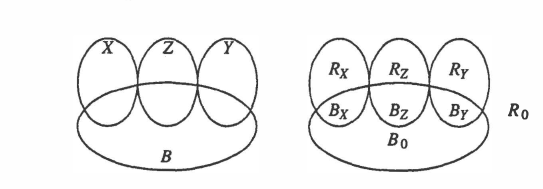
\includegraphics[scale=0.6]{imgs/img7.png}
	\end{center}
	\caption{Case 2}
	\label{fig:case2}
\end{figure}

By construction, there is an edge from all vertices \( B \) to \( n \). Since \( T \in M_G \), any path between \( n \) and \( Y \) must be blocked by \( Z \), so \( B_Y = \emptyset \), otherwise there would be a path consisting of just one edge from \( b \in B_Y \) to \( n \). Thus, \( Y = R_Y \), and the last triplet of the protocol can be represented as \( (n, B_X B_0 B_Z, R_X R_Z R_0 Y) \).

Since \( M \) is a semi-graphoid, by the weak union property, we can move \( R_X R_Z \) from the third element of the triplet to the second and obtain a valid independence relation: \( (n, B R B_0, Y R_0) \in M \). Also, by decomposition, we can ignore \( R_0 \) in the last element of the triplet and again obtain an element of \( M \):

\begin{align}
	(n, X Z B_0, Y) \in M
	\label{eq:case2}
\end{align}

All elements \( B_0 \) are connected by an edge to \( n \), and \( n \) is d-separated from \( Y \) by the vertices \( Z \), so \( B_0 \) is also d-separated from \( Y \) by the same \( Z \), since otherwise there would be a path \( B_0 \leadsto Y \), but then, because \( B_0 \rightarrow n \), there would be an unblocked path \( Y \leadsto n \) not blocked by \( Z \). Now, since \( X \) and \( B_0 \) are d-separated from \( Y \) via \( Z \), their union is also separated from \( X \) via \( Z \), so \( (X B_0, Z, Y) \in M_G \). In this triplet, \( n \) does not appear, so by case 1, we have \( (X B_0, Z, Y) \in M \). Combining this with \ref{eq:case2} and using the contraction property, we obtain \( (Y, Z, n X B_0) \in M \), and then by the decomposition property, \( (n X, Z, Y) \in M \).

\textbf{Case 3}: \( T = (X, n Z, Y) \). Again, represent the last element of the stratification protocol as \( (n, B_X B_Y B_Z B_0, R_X R_Y R_Z R_0) \in M \). Note that \( B_X = \emptyset \lor B_Y = \emptyset \), since otherwise there would be a path \( b_x \rightarrow n \leftarrow b_y \), unblocked by conditioning on \( n \), i.e., there would be an unblocked path \( X \leadsto Y \), which would contradict \( T \in M_G \). Without loss of generality, let \( B_Y = \emptyset \). By considerations from the previous point, \( (B_0, Z, Y) \in M_G \).

Further, \( (X, n Z, Y) \in M_G \implies (X, Z, Y) \in M_G \), since \( n \) has only incoming edges, so if there were an unblocked path \( X \leadsto Y \) not blocked by \( Z \), conditioning on \( n \) would not help block it. Thus, \( (X B_0, Z, Y) \in M_G \), and by case 1, also \( (X B_0, Z, Y) \in M \). By reasoning from case 2, the last triplet of the protocol can be represented as \( (n, B_X B_0 B_Z, R_X R_Z R_0 Y) \in M \) and ultimately \( (n, X Z B_0, Y) \in M \implies (n X B_0, Z, Y) \in M \implies (X B_0, n Z, Y) \implies (X, n Z, Y) \) (weak union, then decomposition).

\textbf{Case 4}: \( T = (X, Z, n Y) \) - by symmetry, reduces to case 2.

\(\blacksquare\)

\begin{tcolorbox}
	In essence, how to use this theorem, that is, what are the implications? Here they are: suppose there is a dependency model (any semi-graphoid), and we have constructed some stratification protocol \( L_\theta \) for it, and from the stratification protocol, we have constructed a DAG. So, any d-separation of sets in the DAG means the membership of the corresponding triple (conditional independence) in the dependency model.
\end{tcolorbox}

Another simple corollary: if the stratification protocol \( L_\theta \) of the dependency model \( M \) is such that all tail boundaries in it are minimal (no element can be removed from any of them without violating the membership of the triplet in \( M \)), then the DAG constructed from this protocol is a minimal I-map of the model—obviously, it is an I-map by the theorem, and minimal because each edge is determined by some tail boundary of the protocol, meaning no edge can be removed without violating the I-map (otherwise, we would reconstruct from the truncated DAG back to the truncated stratification protocol, and it would be correct).

Returning to the original theorem about the consequences of d-separation in the context of probability distributions: we have shown that if \( P(V) \) is Markov relative to the DAG \( G \), then \( X \indepg Y | Z \implies X \independent Y | Z \). Well, because in this case, \( P(V) \) acts as a dependency model, and Markov compatibility allows constructing a stratification protocol of this model corresponding to \( G \). But nothing has been done yet with the second statement of the theorem: that if in the graph there is no d-separation of sets \( X, Y \) by set \( Z \), then there exists a distribution compatible with \( G \) in which \( X \not\independent Y | Z \). For now, let's leave this fact unproven.

\begin{theorem} \textbf{Ordered Markov Condition}\\
	A necessary and sufficient condition for the distribution \( P \) to be Markov compatible with \( G \) is that each variable is independent of all its predecessors in some ordering consistent with \( G \) when conditioned on its parents in \( G \).
	\label{th:ordered_markov}
\end{theorem}

\textbf{Necessity}: Let \( P \) be compatible with \( G \). This means that \( P(x_1..x_n) = \prod P(x_i|pa_i) \). Order the variables using topological sorting according to the graph \( G \). We need to show that \( P(x_i | pa_i, x_j) = P(x_i | pa_i) \).

Note that

\begin{align}
	P(x_1...x_n) = \prod\limits_{k\le i}P(x_k|pa_k)\prod\limits_{k> i} P(x_k | pa_k)
	\label{eq:factorization1}
\end{align}

From this, the marginal distribution of the first \( i \) variables in our chosen order is easily derived by summing the equality

\begin{align}
	\begin{split}
		P(x_1...x_i) &= \prod\limits_{k\le i}P(x_k|pa_k)\sum\limits_{x_j: j > i}\prod\limits_{k> i} P(x_k | pa_k)\\
		&= \prod\limits_{k\le i}P(x_k|pa_k)\sum\limits_{x_j : i < j < n}\prod\limits_{ i < k < n}P(x_k | pa_k) \sum\limits_{x_n}P(x_n | pa_n)\\
		&= \ldots = \prod\limits_{k\le i}P(x_k|pa_k)
		\label{eq:factorization2}
	\end{split}
\end{align}

Using \ref{eq:factorization2}, we easily derive the relation

\begin{align}
	P(x_i|x_1,...,x_{i-1}) = \frac{P(x_1,...,x_i)}{P(x_1,...,x_{i-1})} = \frac{\prod\limits_{k\le i}P(x_k|pa_k)}{\prod\limits_{k\le i - 1}P(x_k|pa_k)} = P(x_i|pa_i)
\end{align}

Thus, \( X_i \independent \{x_1...x_{i-1}\} \backslash PA_i\ |\ PA_i \). We have already proven earlier that the conditional independence relation for a set of random variables forms a graphoid, and therefore, by the decomposition property, \( \forall j < i: X_j \notin PA_i \implies X_i \independent X_j | PA_i \), which is what was required.

\textbf{Sufficiency}: Let each variable \( X_i \) be independent of all variables with a smaller number when conditioned on the immediate ancestors of the variable in the graph \( G \). Let us show that in this case, the distribution is Markov compatible with \( G \), i.e., that it factorizes according to \( G \).

Any distribution can be represented in the following factorization:

\begin{align}
	P(x_1,...,x_n) = \prod\limits_i P(x_i|x_1,...,x_{i-1})
\end{align}

Note that now it remains for us to use the condition that each variable is conditionally independent of all variables with a smaller number when conditioned on its parents in the graph \( G \), to obtain the necessary equality:

\begin{align}
	P(x_1,...,x_n) = \prod\limits_i P(x_i|pa_i)
\end{align}

\(\blacksquare\)

Another similar theorem:

\begin{theorem} \textbf{Parental Markov Condition}\\
	A necessary and sufficient condition for the distribution \( P \) to be Markov compatible with \( G \) is that each variable is independent of all its \textit{non-descendants} in some ordering consistent with \( G \) when conditioned on its parents in \( G \).
\end{theorem}

\textbf{Necessity}: Let \( P(v) \) be compatible with the graph \( G \), and \( x_j \notin de(x_i) \). Let us show that \( x_i \independent x_j \ |pa_i \). Note that if \( j < i \), then the statement follows from the previous theorem on the ordered Markov condition. Let \( j > i \). Clearly, in the graph \( G \), there is no directed path \( x_i \leadsto x_j \) (since \( x_j \notin de(x_i) \)), nor a directed path \( x_j \leadsto x_i \), since in this case, the ordering of the variables would not be consistent with the graph topology. Therefore, in any path connecting \( x_i \) and \( x_j \), there is at least one connection of the form \( \rightarrow x_k \leftarrow \), and of course \( x_k \notin pa_i \), since then there could not be two arrows in the path. But any such path is blocked by the set \( pa_i \), so \( x_i \) and \( x_j \) are d-separated in \( G \) by the set \( pa_i \), and therefore, conditionally independent when conditioned on \( pa_i \) according to the probabilistic consequences of d-separation.

\textbf{Sufficiency}: Here everything is simple: if each variable is independent of its non-descendants, then it is certainly independent of all variables with smaller numbers than its own, and therefore, by the previous theorem, the distribution is compatible with \( G \).

\(\blacksquare\)

\define{Observational Equivalence} Two graphs are called observationally equivalent if any distribution compatible with the first is compatible with the second, and vice versa.

\begin{theorem} \textbf{On Observational Equivalence}\\
	Two graphs are observationally equivalent if and only if they have the same skeleton and set of \( v \)-structures.
\end{theorem}

\textbf{Necessity}: Let two graphs be observationally equivalent. Let us prove that they have the same skeleton and set of v-structures.

Let's start with the skeleton. Suppose the graph \( G_1 \) has an edge \( x-y \), and \( G_2 \) does not. Consider the following distribution:

\begin{align}
	P(x_1,..x_n) = uniform_{[0,1]}(x)bernoulli_x(y)
\end{align}

where all variables except the two under consideration are constant. Note that such a distribution will be compatible with \( G_1 \), as it factorizes according to it. At the same time, it is not compatible with \( G_2 \). Indeed, suppose it is compatible. According to the ordered Markov condition theorem \ref{th:ordered_markov}, in this case, there exists an ordering consistent with \( G_2 \) in which each variable is independent of variables with smaller numbers when conditioned on its parents in \( G_2 \). Without loss of generality, assume that \( x \) is ordered before \( y \). Note that \( x \notin PA_y \), since there is no edge between them in \( G_2 \), so \( P(y|x) = \sum_{pa_y} P(y, pa_y|x) = \sum_{pa_y} P(y|x, pa_y) P(pa_y|x) = \sum_{pa_y} P(y|pa_y) = P(y) \), i.e., \( y \) should be independent of \( x \) in \( P \), but this is not the case. We have arrived at a contradiction, so \( P \) is incompatible with \( G_2 \), but then \( G_1 \) and \( G_2 \) are observationally nonequivalent, which contradicts the initial assumption, so \( G_2 \) also does not have the edge \( x-y \). Thus, the skeletons of the graphs coincide.

Now let's prove that the graphs have the same v-structures. Well, this is quite simple to prove: consider any two such graphs, and assume the statement is false. We already know that the skeletons of the graphs coincide, so the undirected paths also coincide. If the sets of v-structures do not coincide, there is at least one path \( x \leadsto y \), blocked by \( Z \) in the first graph and unblocked in the second (the symmetric case is analogous). Consider this path in both graphs. The difference in blocking can only be due to the different orientation of arrows at some vertex \( v \). There are only four ways to orient arrows in a path:

1. \( ...\rightarrow v \leftarrow ... \), but in this case, \( v \) has the same arrows in both graphs, as it is a vertex of a v-structure, so this vertex cannot distinguish the blocking of the path in the graphs.

2. \( \rightarrow v \rightarrow \)

3. \( \leftarrow v \leftarrow \)

4. \( \leftarrow v \rightarrow \)

The last three options can be observed in both graphs independently. However, in any combination, if \( v \in Z \), then in both graphs \( v \) blocks the path, and if \( v \notin Z \), it does not block. That is, in any case, any valid direction of arrows in \( v \) cannot distinguish the blockedness of the path in the graphs, so the assumption is incorrect.

\textbf{Sufficiency}: Let two graphs have the same skeleton and set of v-structures. We need to show that they are observationally equivalent.

This will require some effort. We will prove by induction on the number of vertices in the graphs. With one vertex, everything is clear and true, so we assume that the base exists.

Suppose we have proved the statement for all graphs with fewer than \( n \) vertices. Consider two graphs on \( n \) vertices with the same skeleton and set of v-structures. Suppose \( P(v) \) is compatible with \( G_1 \), and let us show that it is then also compatible with \( G_2 \).

\begin{figure}[h]
	\begin{center}
		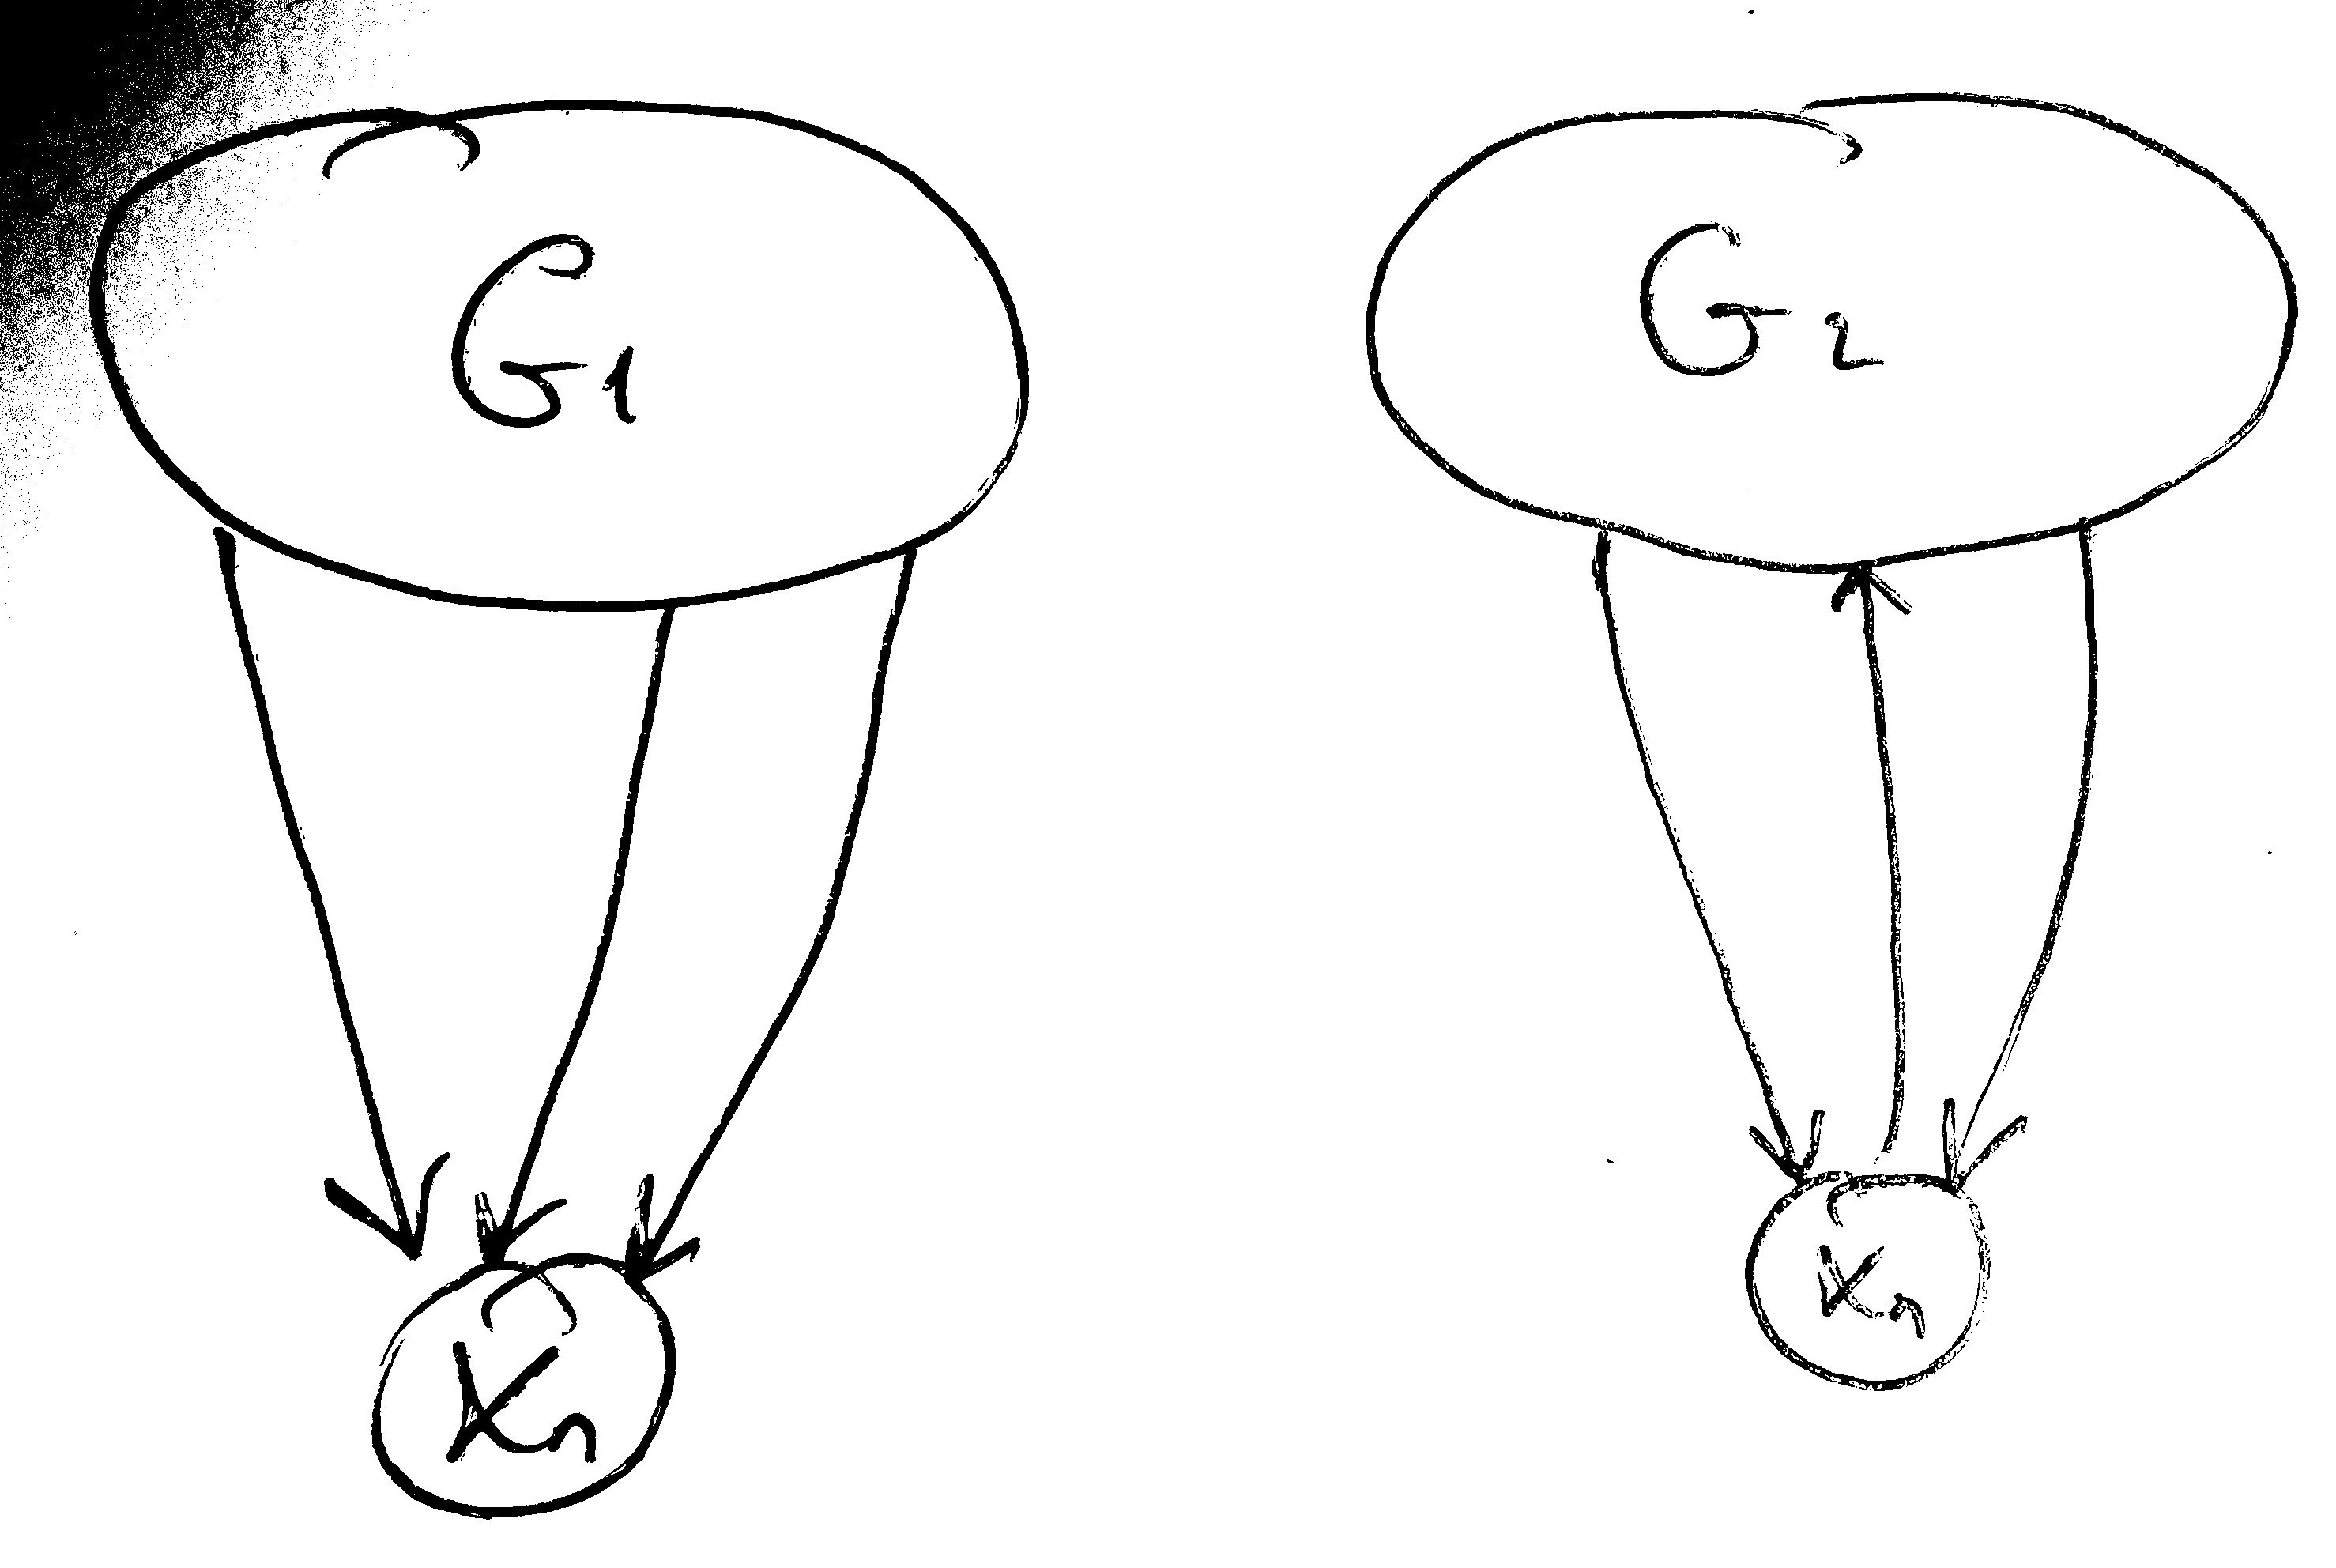
\includegraphics[scale=0.1]{imgs/img10.png}
	\end{center}
	\caption{The two considered graphs \( G_1 \) and \( G_2 \)}
	\label{fig:equiv1}
\end{figure}

Since \( P(v) \) is compatible with \( G_1 \), it factorizes according to it:

\begin{align}
	P(x_1,...x_n) = \prod\limits_{i}P(x_i|pa^1_{i})
\end{align}
	
\end{document}